
\documentclass{article}

\usepackage[ngerman]{babel}                     %for german umlauts
\usepackage[utf8]{inputenc}
\usepackage{subfigure}
% \usepackage[ansinew]{inputenc}        %for german umlauts

\usepackage{graphicx}
\usepackage{hyperref}

\usepackage{amssymb}    %for different fonts
\usepackage{amsmath}
% Geht nicht: \usepackage{bbm}
% \usepackage[usenames,dvips]{color} %only way to get it running with pdf:(
% \usepackage[pdftex,usenames,dvipsnames]{color}        % does not work
% \usepackage{color}
\usepackage{verbatim}
\usepackage{polynom}

\setlength{\parindent}{0pt}
\addtolength{\hoffset}{-1cm}
\addtolength{\voffset}{-1cm}
\addtolength{\textheight}{3cm}
\addtolength{\textwidth}{1cm}

\newcommand{\im}{\operatorname{Im}}
\newcommand{\rg}{\operatorname{rg}}
\newcommand{\ggt}{\operatorname{ggT}}

\begin{document}

\section*{\begin{center} Mustererkennung - Aufgabenblatt 02 \end{center}}
\begin{center}
  André Hacker und Dimitri Schachmann \\
\end{center}


\subsection*{1. Visualisierung}
Wir haben mit Matlab die Mittlewerte der Daten berechnet und sie so
wie beim ersten Übungsblatt mit gnuplott dargestellt. Die Startpunkte
sind mt Kreisen gekennzeichnet.

\begin{figure}[h!]
  \begin{subfigure}
    \centering
    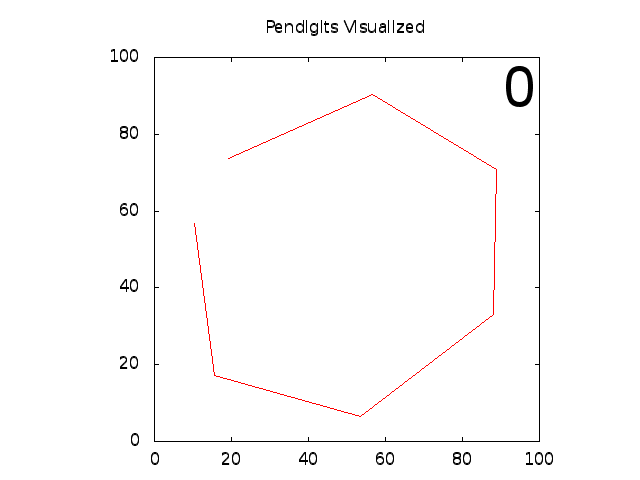
\includegraphics[scale=0.3,bb=0 0 640 480]{images/mean0.png}
    \label{picture-label}
  \end{subfigure}
  \begin{subfigure}
    \centering
    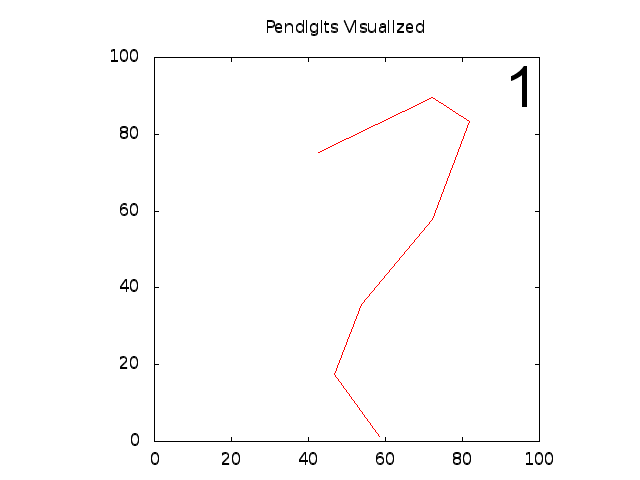
\includegraphics[scale=0.3,bb=0 0 640 480]{images/mean1.png}
    \label{picture-label}
  \end{subfigure}
  \begin{subfigure}
    \centering
    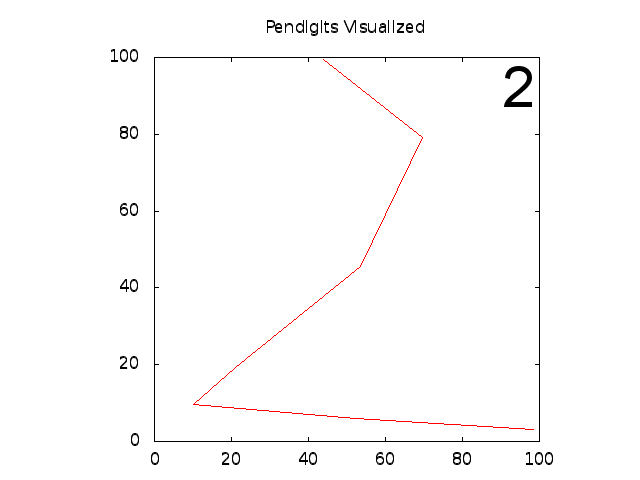
\includegraphics[scale=0.3,bb=0 0 640 480]{images/mean2.png}
    \label{picture-label}
  \end{subfigure}
  \begin{subfigure}
    \centering
    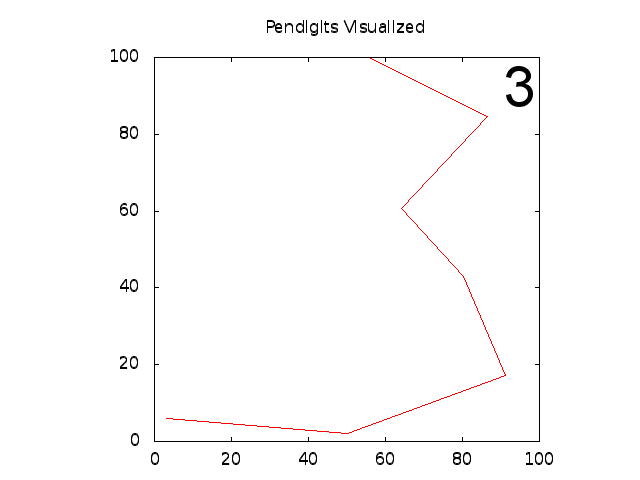
\includegraphics[scale=0.3,bb=0 0 640 480]{images/mean3.png}
    \label{picture-label}
  \end{subfigure}
  \begin{subfigure}
    \centering
    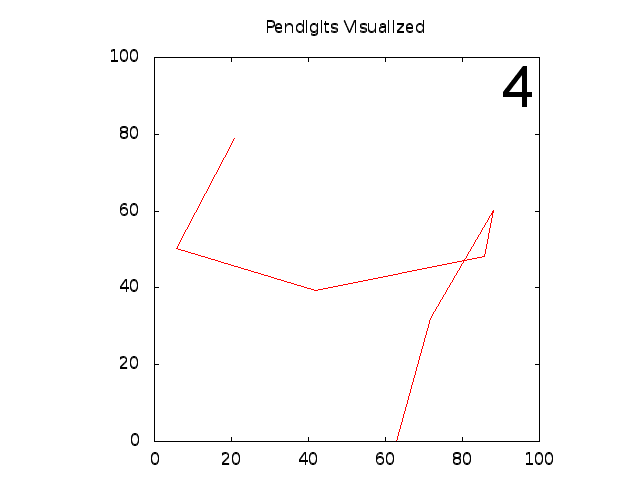
\includegraphics[scale=0.3,bb=0 0 640 480]{images/mean4.png}
    \label{picture-label}
  \end{subfigure}
  \begin{subfigure}
    \centering
    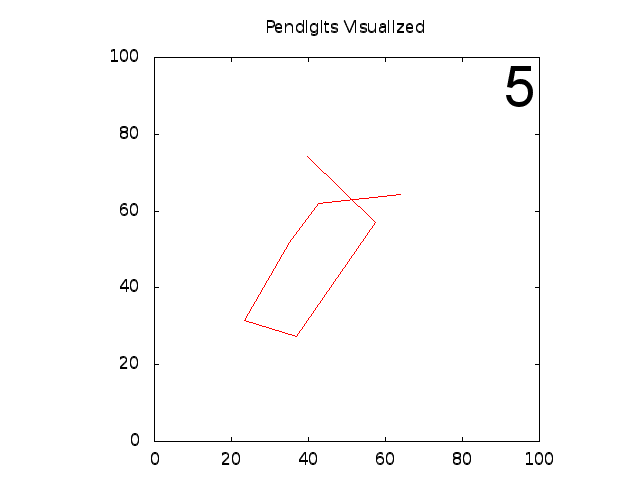
\includegraphics[scale=0.3,bb=0 0 640 480]{images/mean5.png}
    \label{picture-label}
  \end{subfigure}
\end{figure}
\begin{figure}[h!]
  \begin{subfigure}
    \centering
    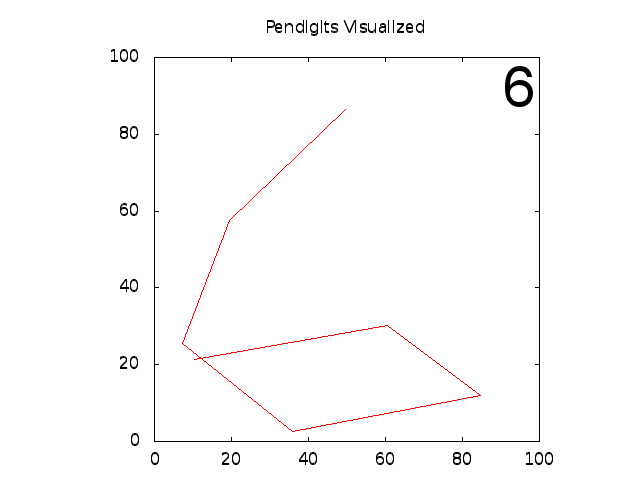
\includegraphics[scale=0.3,bb=0 0 640 480]{images/mean6.png}
    \label{picture-label}
  \end{subfigure}
  \begin{subfigure}
    \centering
    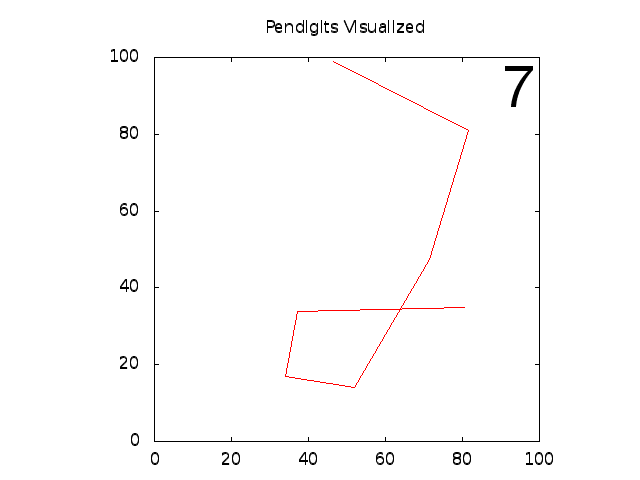
\includegraphics[scale=0.3,bb=0 0 640 480]{images/mean7.png}
    \label{picture-label}
  \end{subfigure}
  \begin{subfigure}
    \centering
    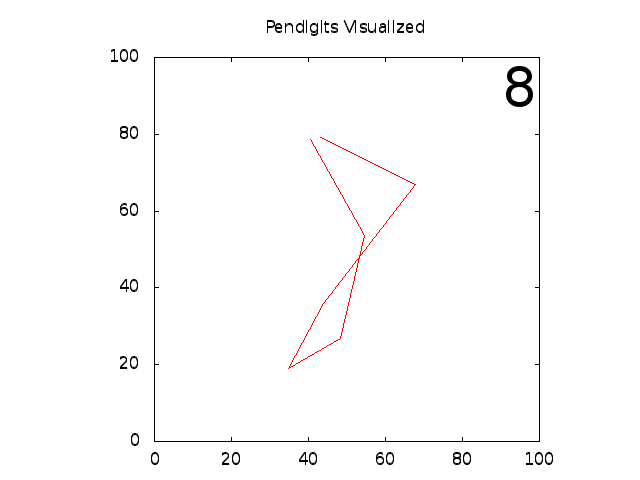
\includegraphics[scale=0.3,bb=0 0 640 480]{images/mean8.png}
    \label{picture-label}
  \end{subfigure}
  \begin{subfigure}
    \centering
    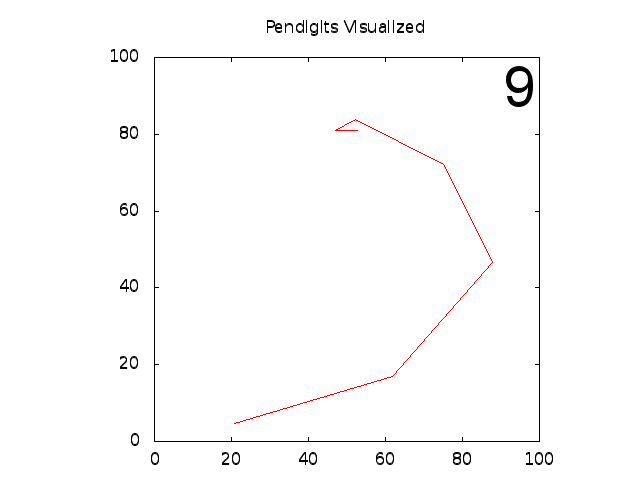
\includegraphics[scale=0.3,bb=0 0 640 480]{images/mean9.png}
    \label{picture-label}
  \end{subfigure}
\end{figure}





\subsection*{2. Klassifikation}
\subsubsection*{a) Mit cov, mean und mvnpdf}
Wir haben die Klassifikation mittels der multivariaten
Normalverteilung in Matlab implementiert. Zunächst haben wir das mit
Hilfe der Matlab funktionen \textbf{cov}, \textbf{mean} und
\textbf{mvnpdf} implementiert, was sehr einfach war:

\verbatiminput{covar.m}

\subsubsection*{b) Ohne cov und mvpdf}
Dann haben wir das ganze noch mal mit eigener Kovarianz, Mittelwert
und Dichtefunktion implementiert:

\verbatiminput{covar2.m}

\subsubsection*{c) Erkennungsrate und Confusion Matrix}
Die Erkennungsrate dies Algorithmus ist 95.9\%, was wir für
überraschend gut halten. Wenn man bedenkt, dass der Algorithmus aus
dem 1. Übungsblatt (zumindest bei uns) eine viertel Stunde gelaufen
ist und mit 97.4\% nur unwesentlich besser war, während dieser in 1
Sekunde fertig ist.

\begin{table}[h!]
  \begin{tabular}{|l|l|l|l|l|l|l|l|l|l|l|}
    \hline
    & 0   & 1   & 2   & 3   & 4   & 5   & 6   & 7   & 8   & 9   \\
    \hline
    0 & 341 & 0   & 0   & 0   & 0   & 0   & 0   & 0   & 22  & 0   \\
    1 & 0   & 350 & 12  & 0   & 1   & 0   & 0   & 0   & 1   & 0   \\
    2 & 0   & 8   & 355 & 0   & 0   & 0   & 0   & 1   & 0   & 0   \\
    3 & 0   & 9   & 0   & 320 & 0   & 1   & 0   & 1   & 0   & 5   \\
    4 & 0   & 0   & 0   & 0   & 362 & 0   & 0   & 0   & 0   & 2   \\
    5 & 0   & 0   & 0   & 1   & 0   & 323 & 0   & 0   & 2   & 9   \\
    6 & 0   & 0   & 0   & 0   & 0   & 0   & 325 & 0   & 11  & 0   \\
    7 & 0   & 28  & 0   & 0   & 0   & 0   & 0   & 314 & 5   & 17  \\
    8 & 0   & 0   & 0   & 0   & 0   & 0   & 0   & 0   & 336 & 0   \\
    9 & 0   & 5   & 0   & 0   & 0   & 0   & 0   & 1   & 1   & 329 \\
    \hline
  \end{tabular}
\end{table}

\subsection*{3. Code für die Visualisierung}
Für die Visualisierung der Ziffern haben wir ein einfaches gnuplot
Skript geschrieben:
\verbatiminput{visual.gnu}

\end{document}
